\documentclass[a4, 12pt]{article}
\usepackage[a4paper,top=1.3cm,bottom=2cm,left=1.5cm,right=1.5cm,marginparwidth=0.75cm]{geometry}
\usepackage{setspace}
\usepackage{cmap}
\usepackage{mathtext}
\usepackage[utf8]{inputenc}
\usepackage[english,russian]{babel}
\usepackage[T2A]{fontenc}
\usepackage{multirow}
\usepackage{graphicx}
\usepackage{wrapfig}
\usepackage{tabularx}
\usepackage{float}
\usepackage{longtable}
\usepackage{hyperref}
\hypersetup{colorlinks=true,urlcolor=blue}
\usepackage[rgb]{xcolor}
\usepackage{amsmath,amsfonts,amssymb,amsthm,mathtools}
\usepackage{icomma}
\mathtoolsset{showonlyrefs=true}
\usepackage{euscript}
\usepackage{mathrsfs}

\DeclareMathOperator{\sgn}{\mathop{sgn}}
\newcommand*{\hm}[1]{#1\nobreak\discretionary{}
	{\hbox{$\mathsurround=0pt #1$}}{}}


\title{\textbf{Определение моментов инерции твердых тел с помощью трифилярного подвеса. (1.2.3)}}
\author{Балдин Виктор Б01-303}
\date{30 октября 2023}


\begin{document}

	\maketitle

	\section{Введение}

	\textbf{Цели работы:} измерение момента инерции тел и сравнение результатов с расчетами по теоретическим формулам; проверка аддитивности моментов инерции и справедливости формулы Гюйгенса-Штейнера.\\
	\textbf{Оборудование:} трифилярный подвес, секундомер, счетчик числа колебаний, набор тел, момент инерции которых надлежит измерить (диск, стержень, полный цилиндр и другие).
	\section{Теоретические сведения}

	\par Инерционность при вращении тела относительно оси определяется моментом инерции тела относительно этой оси. Момент инерции твердого тела относительно неподвижной оси вращения вычисляется по формуле:

	\begin{equation}
		I = \int r^2 dm
	\end{equation}

	Здесь $r$ -- расстояние элемента массы тела $dm$ от оси вращения. Интегрирование проводится по всей массе тела $m$.

	Если пренебречь потерями энергии на трение о воздух и крепление нитей, то уравнение сохранения энергии при колебаниях можно записать следующим образом:

	\begin{equation}\label{moment}
		\frac{I \dot{\varphi^2}}{2} + mg(z_0-z) = E
	\end{equation}

	Здесь $I$ -- момент инерции платформы вместе с исследуемым телом, $m$ -- масса платформы с телом, $\varphi$ -- угол поворота платформы от положения равновесия системы, $z_0$ -- координата по вертикали центра нижней платформы $O'$  при равновесии ($\varphi = 0$), $z$ -- координата той же точки при некотором угле поворота $\varphi$. Правый член в левой части уравнения -- кинетическая энергия вращения, второй член -- потенциальная энергия в поле тяжести, $E$ -- полная энергия системы (платформы с телом).

	Воспользуемся системой координат $x, y, z$, связанной с верхней платформой, как показано на Рис. \ref{risunok}. Координаты верхнего конца одной из нитей подвеса точки $C$ в этой системе -- $(r, 0, 0)$. Нижний конец данной нити $C'$, находящийся на нижней платформе, при равновесии имеет координаты $(R, 0, z_0)$, а при повороте платформы на угол $\varphi$ эта точка переходит в $C''$ с координатами $(Rcos\varphi, Rsin\varphi, z)$. расстояние между точками $C$ и $C''$ равно длине нити, поэтому, после некоторых преобразований, получаем:

	\begin{center}
	\begin{spacing}{1.6}
		$ (R\cos\phi - r)^2 + R^2\sin^2\phi + z^2 = L^2 $

		$ z^2 = L^2 - R^2 - r^2 + 2Rr\cos\phi \approx z^2_{0} - 2Rr(1 - \cos\phi) \approx z^2_{0} - Rr\phi^2 $

		$ z = \sqrt{z^2_{0} - Rr\phi^2} \approx z_{0} - \frac{Rr\phi^2}{2z_{0}} $
	\end{spacing}
	\end{center}

	Подставляя $z$ в уравнение \eqref{moment}, получаем:

	\begin{equation}
		\frac{1}{2}I\dot{\varphi^2} + mg \frac{Rr}{2z_0}\varphi^2 = E
	\end{equation}

	Дифференцируя по времени и сокращая на $\dot\varphi$, находим уравнение крутильных колебаний системы:

	\begin{equation}
		I\ddot\varphi^2 + mg\frac{Rr}{2z_0}\varphi^2 = 0
	\end{equation}

	Производная по времени от $E$ равна нулю, так как потерями на трение, как уже было сказано выше, пренебрегаем.

	Решение этого уравнения имеет вид:

	\begin{equation}
		\varphi = \varphi_0 \sin \left(\sqrt{\frac{mgRr}{Iz_0}}t + \theta\right)
	\end{equation}

	Здесь амплитуда $\varphi_0$ и фаза $\theta$ колебаний определяются начальными условиями. Период крутильных колебаний нашей системы равен:

	\begin{equation}
		T = 2\pi \sqrt{\frac{Iz_0}{mgRr}}
	\end{equation}

	Из формулы для периода получаем:

	\begin{equation}\label{momin}
		I = \frac{mgRrT^2}{4 \pi^2z_0} = kmT^2
	\end{equation}

	\section {Методика измерений}

	\begin{wrapfigure}{l}{7cm}
		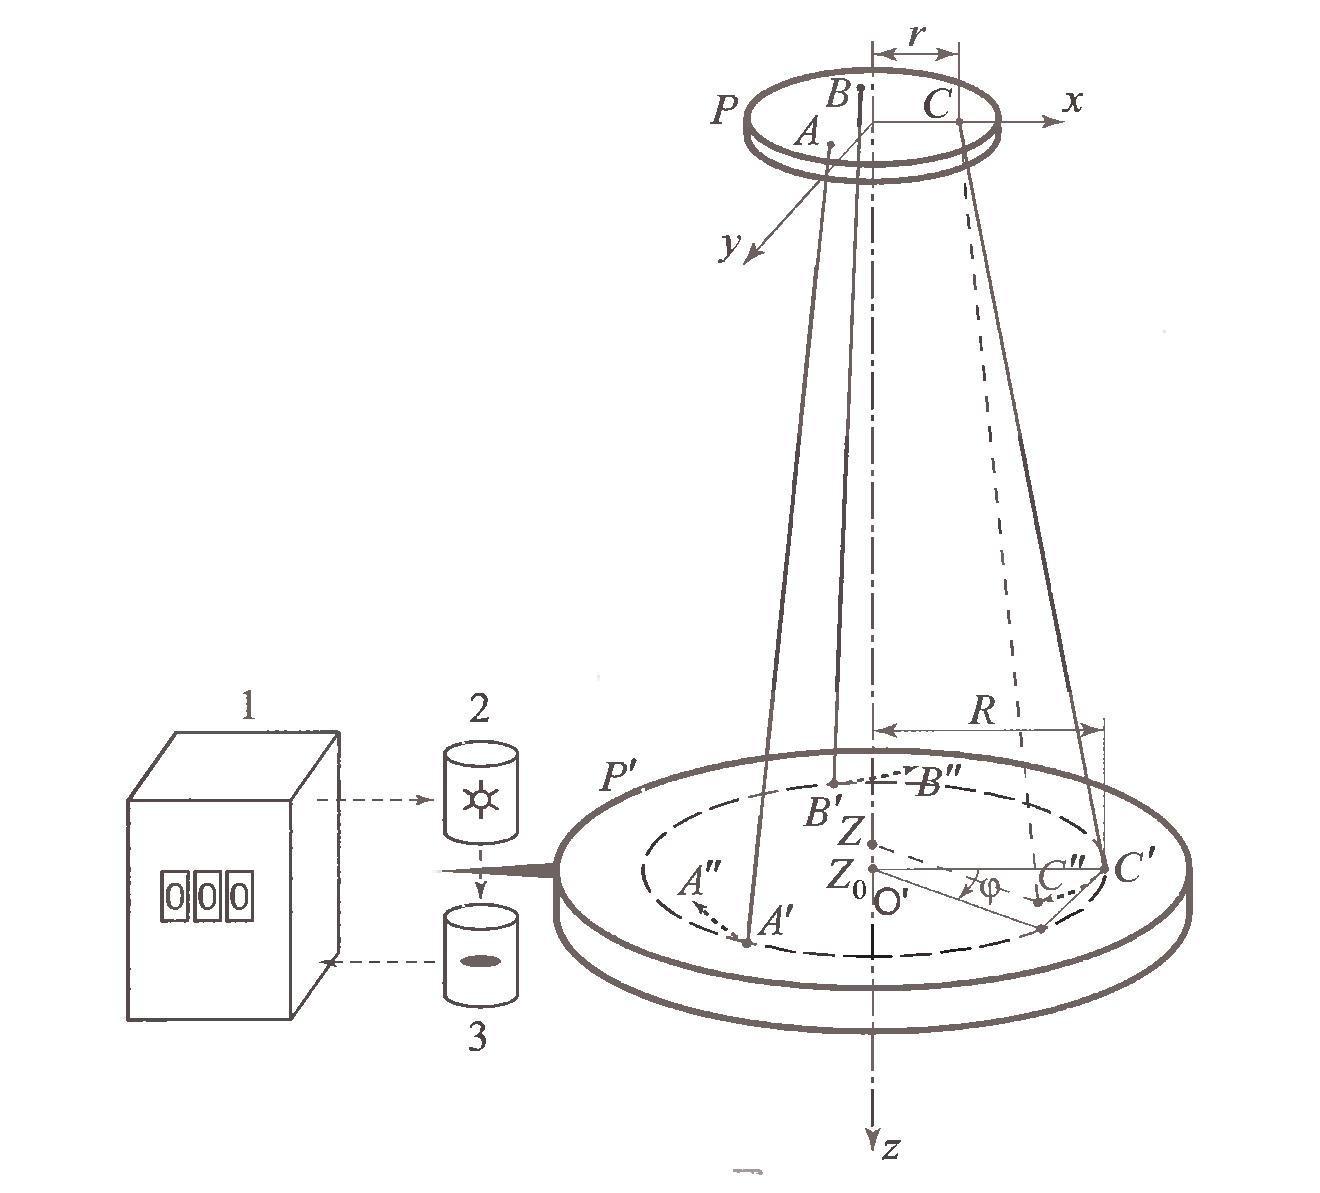
\includegraphics[width=0.95\linewidth]{1.2.3 ustan.png}
		\caption{Физический маятник}\label{risunok}
	\end{wrapfigure}

	Для наших целей удобно использовать устройство, показанное на Рис. \ref{risunok} и называемое трифилярным подвесом. Оно состоит из укрепленной на некоторой высоте неподвижной платформы $P$ и подвешенной к ней на трех симметрично расположенных нитях $AA'$, $BB'$ и $CC'$, вращающейся платформы $P'$.

	Чтобы не вызывать дополнительных раскачиваний, лучше поворачивать верхнюю платформу, укрепленную на неподвижной оси. После поворота верхняя платформа остается неподвижной в течение всего процесса колебаний. После того, как нижняя платформа $P'$ оказывается повернутой на угол $\varphi$ относительно верхней платформы $P$ возникает момент сил, стремящийся вернуть нижнюю платформу в положение равновесия, при котором относительный поворот платформ отсутствует. В результате платформа совершает крутильные колебания.

	\noindent где $k = \frac{gRr}{4\pi^2z_0}$ -- величина, постоянная для данной установки.

	\section{Оборудование}
	Трифилярный подвес, секундомер, счетчик числа колебаний, набор тел, момент инерции которых надлежит измерить (диск, стержень, полный цилиндр и другие).

	\section{Результаты измерений и обработка данных}
	\begin{enumerate}
		\item Проверим исправность установки.
		\item Измерим параметры установки:
		$$ z_0 = (213.6\pm0.5) \;\text{см} $$
		$$ R = (114.6\pm0.5) \;\text{мм} $$
		$$ r = (30.2\pm0.3) \;\text{мм}  $$
		$$ m = (1066.8\pm0.5) \;\text{г} $$
		\item Вычислим $k$:
		$$ k = \frac{gRr}{4\pi^2z_0} = 4.43\cdot10^{-4} \;\text{кг}\cdot\text{м}$$
		$$ \varepsilon_k = \varepsilon_R + \varepsilon_r + \varepsilon_{z_0} = 0.02 $$
		$$ k = (4.43\pm0.09)\cdot10^{-4} \;\text{кг}\cdot\text{м}$$
		\item Вычислим момент инерции пустой платформы.
		$$ I = \frac{mR^2}{2} = 7.264\cdot10^{-3} \;\text{кг}\cdot\text{м} $$
		$$ \varepsilon_I = 2\varepsilon_R + \varepsilon_m = 0.01 $$
		$$ I = (7.264\pm0.073)\cdot10^{-3}\;\text{кг}\cdot\text{м} $$
		\item Перейдем к измерению моментов инерции данных нам тел.
		Для кольца получим:
		\begin{table}[H]
			\centering
			\begin{tabular}{|c|c|c|c|}
			\hline
			$t$, c & $T$, c & $I_t+I$, $10^{-3}$ кг$\cdot$м$^2$ & $I_t$, $10^{-3}$, кг$\cdot$м$^2$ \\ \hline
			126.08 & 4.203  & 12.97                             & 5.15                             \\ \hline
			125.94 & 4.198  & 12.94                             & 5.12                             \\ \hline
			126.55 & 4.218  & 13.06                             & 5.25                             \\ \hline
			\end{tabular}
			\end{table}
			По итогу получим $I_\text{кол} = (5.17\pm0.08)\cdot10^{-3}$ кг$\cdot$м$^2$.
		\item
    Сделаем все то же самое для диска с параметрами
    \begin{align*}
    m_{диск} &= (580.6 \pm 0.5) \;\text{г} \\
    r_{диск} &= (5.75 \pm 0.01) \;\text{см}
    \end{align*}

    \begin{table}[h!]
    \begin{center}
    \begin{tabular}{|l|r|r|r|}
    \hline
    No &   N &       t, с &         T, с \\
    \hline
    1  &  10 &  39.254 &  3.9254 \\
    2  &  10 &  39.221 &  3.9221 \\
    3  &  10 &  39.203 &  3.9203 \\
    4  &  10 &  39.189 &  3.9189 \\
    \hline
    \end{tabular}
    \end{center}
    \end{table}
    Из этих данных получаем



    Теоретически получаем
    \[I^{теор}_{диск} = m_{диск}r_{диск}^2 = (1.920 \pm 0.007)\cdot10^{-3}\;\text{кг}\cdot\text{м}^2\]
    Как видим в пределах погрешности теория соответствует эксперименту.

    \paragraph{}
    Когда оба тела на платформе.

    \begin{table}[h!]
    \begin{center}
    \begin{tabular}{|l|r|r|r|}
    \hline
    No &   N &       t, с &         T, с \\
    \hline
    1  &  10 &  39.750 &  3.9750 \\
    2  &  10 &  39.873 &  3.9873 \\
    3  &  10 &  39.964 &  3.9964 \\
    4  &  10 &  39.773 &  3.9773 \\
    \hline
    \end{tabular}
    \end{center}
    \end{table}

    \begin{align*}
    T &= (3.984 \pm 0.006)\;\text{c} \\
    I_\text{пф+общ}&=(16.4 \pm 0.3)\cdot10^{-3}\;\text{кг}\cdot\text{м}^2 \\
    I_\text{общ}&=(8.7 \pm 0.4)\cdot10^{-3}\;\text{кг}\cdot\text{м}^2 \\
    I_\text{диск} + I_\text{кол}  = (8.8 \pm 0.6)\cdot10^{-3}\;\text{кг}\cdot\text{м}^2
    \end{align*}
	\item Теперь исследуем зависимость момента инерции двух полукругов от расстояния между ними:
			\begin{figure}[H]
			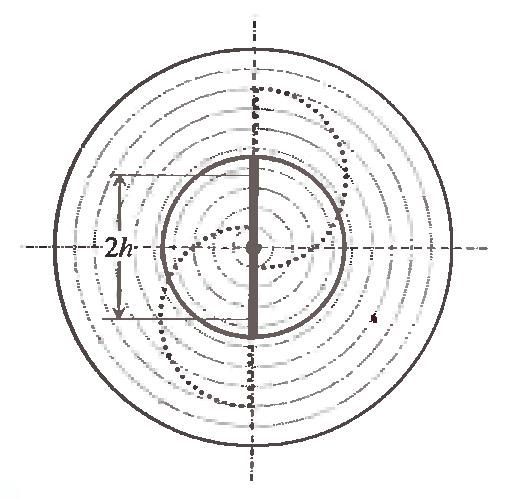
\includegraphics[width=0.25\textwidth]{position}
			\caption{Схема расположения грузов на платформе трифилярного подвеса.}
			\label{ris:position}
		\end{figure}

		Перейдем к определению зависимости момента инерции системы двух тел от их взаимного расположения. Для этого, располагая грузы как показано на рис. \ref{ris:position}, получим зависимость периода от расстояния. Затем, определим зависимость $ I(h^{2}) $

		Полученные результаты измерений занесем в таблицы \ref{tab:period},\ref{tab:moment} соответсвенно. Основывыаясь на результатах таблицы \ref{tab:moment}, построим график зависимости $ I(h^{2}) $. (Рис. \ref{ris:grafik})


		\begin{table}[H]
			\begin{center}
				\begin{tabular}{| l | l | l || l | l | l |}
					\hline
					№ изм. & T, с & h, сm & № изм. & T, с & h, сm \\ \hline
					1 & 3,122 & 0 & 8 & 3,399 & 3,5 \\ \hline
					2 & 3,127 & 0,5 & 9 & 3,472 & 4,0 \\ \hline
					3 & 3,146 & 1,0 & 10 & 3,568 & 4,5 \\ \hline
					4 & 3,167 & 1,5 & 11 & 3,662 & 5,0 \\ \hline
					5 & 3,207 & 2,0 & 12 & 3,753 & 5,5 \\ \hline
					6 & 3,255 & 2,5 & 13 & 3,886 & 6,0 \\ \hline
					7 & 3,325 & 3,0 & 14 & 4,002 & 6,5 \\ \hline
				\end{tabular}
				\caption{Зависимость Периода колебаний от расстояния между дисками.}
				\label{tab:period}
			\end{center}
		\end{table}

		\begin{table}[H]
			\begin{center}
				\begin{tabular}{| l | l | l || l | l | l |}
					\hline
					№ изм. & I, $kgm^2 * 10^{-3}$ & h, cm & № изм. & I, $kgm^2 * 10^{-3}$ & h, сm \\ \hline
					1 & 1,678 & 0 & 8 & 1,827 & 3,5 \\ \hline
					2 & 1,681 & 0,5 & 9 & 1,866 & 4,0 \\ \hline
					3 & 1,691 & 1,0 & 10 & 1,918 & 4,5 \\ \hline
					4 & 1,702 & 1,5 & 11 & 1,968 & 5,0 \\ \hline
					5 & 1,724 & 2,0 & 12 & 2,017 & 5,5 \\ \hline
					6 & 1,750 & 2,5 & 13 & 2,089 & 6,0 \\ \hline
					7 & 1,787 & 3,0 & 14 & 2,151 & 6,5 \\ \hline
				\end{tabular}
				\caption{Зависимость Момента инерции от расстояния между дисками.}
				\label{tab:moment}
			\end{center}
		\end{table}

		\begin{figure}[H]


			\begin{center}
				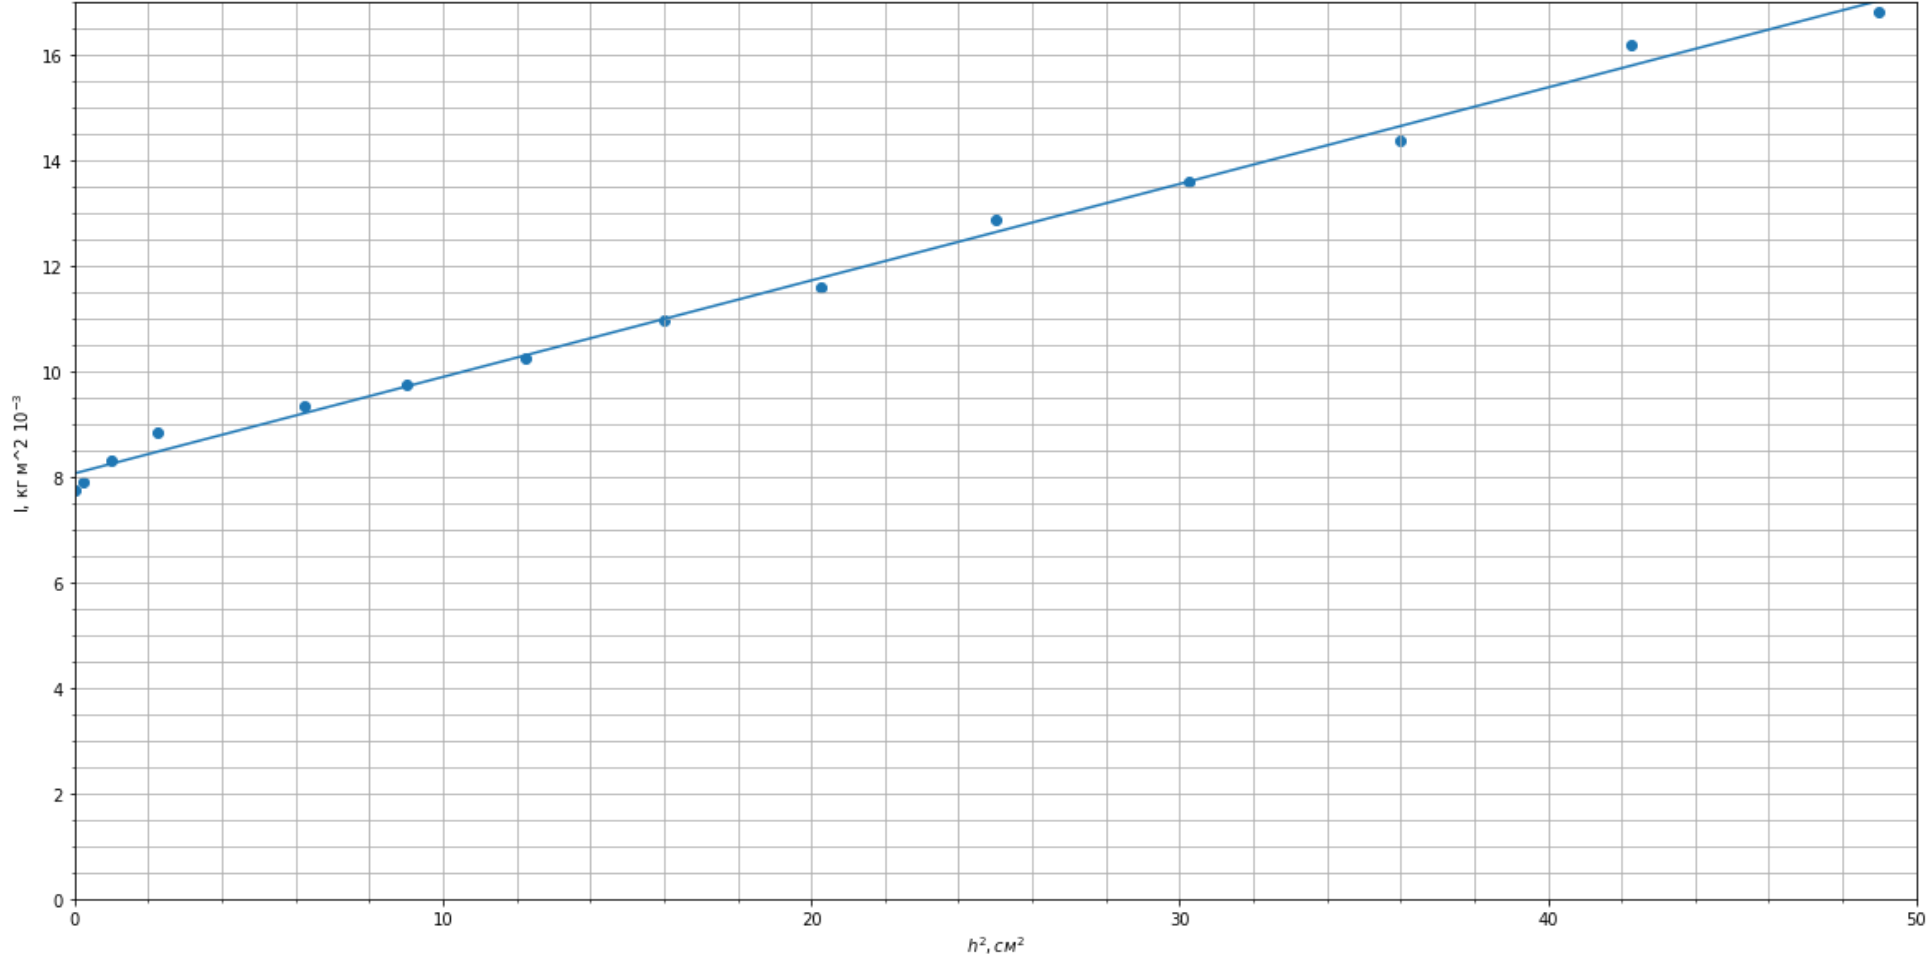
\includegraphics[width=0.9\textwidth]{1.2.3 graph.png}
				\caption{График зависимости $ I(h^2) $}
				\label{ris:grafik}
			\end{center}
		\end{figure}

		Видно, что данная зависимость весьма хорошо аппроксимируется прямой, что согласуется
		с теоретическими данными.

	\end{enumerate}

	\section{Обсуждение результатов}
	\begin{enumerate}
		\item В результате работы были измерены моменты инерции предоставленных тел.
		\item Были посчитаны теоретические моменты инерции и проведено сравнение их
		с экспериментальными результатами. Обнаружено совпадение в пределах погрешности.
		Таким образом, доказана состоятельность метода трифилярного подвеса для
		экспериментального определения моментов инерции различных тел.
		\item Получена экспериментальная зависимость момента инерции системы из двух полукругов
		от расстояния между их центрами инерции. Линеаризованная зависимость $I(h^2)$ действительно
		неплохо аппроксимируется прямой, что очень хорошо согласуется с теорией.
		\item Проверена аддитивность момента инерции системы нескольких тел.
	\end{enumerate}
	\section{Вывод}
	Их проделанной работы можно заключить, что установка на основе трифилярного подвеса хорошо
	подходит для определения моментов инерции тел. Зачастую аналитическое вычисление моментов
	инерции может представлять определенные трудности, особенно в случае сложной и неправильной
	формы тела. В таких случаях приходится прибегать к экспериментальным способам, а значит,
	и считаться с их погрешностями. Как показала практика, опробованный в данной работе метод
	имеет неплохую точность, следовательно, его можно рекомендовать для использования в этих целях.
\end{document}
